\section{Problem 3}
\subsection{Question}
Rerun A9, Q2 but this time using LIBSVM.  If you have n categories,
you'll have to run it n times.  For example, if you're classifying music
and have the categories:\\
\\
metal, electronic, ambient, folk, hip-hop, pop\\
\\
you'll have to classify things as:\\
\\
metal / not-metal\\
electronic / not-electronic\\
ambient / not-ambient\\
\\
etc.\\
\\
Use the 500 term vectors describing each blog as the features, and
your mannally assigned classifications as the true values.  Use
10-fold cross-validation (as per slide 46, which shows 4-fold
cross-validation) and report the percentage correct for 
each of your categories.\\

\subsection{Answer}
The python script in Listing \ref{listing:memfind} was used to retrieve the timemaps and then parse the returned html, traveling down the rabbit hole if the target URI has more than 1000 mementos.
\vspace{1mm}
\lstinputlisting[language=Python, caption={mementofinder.py}, label=listing:memfind]{q3/mementofinder.py}

\vspace{5mm}
The dataset created Listing \ref{listing:memfind}. A log scale was used along the y-axis to show more detail among the results. The script in Listing \ref{listing:bld_hist} was used to create the histogram in Figure \ref{fig:hist_ss}, which shows the difference of mementos per site from the dataset.
\vspace{2mm}
\lstinputlisting[language=R, caption={build\_histogram.r}, label=listing:bld_hist]{q3/build_histogram.r}
\vspace{2mm}
\lstinputlisting[caption=Sample of Memento Links, linerange=7-27]
{q3/site_mementos.txt}
\vspace*{5pt}
\begin{figure}[h]
\centering
\fbox{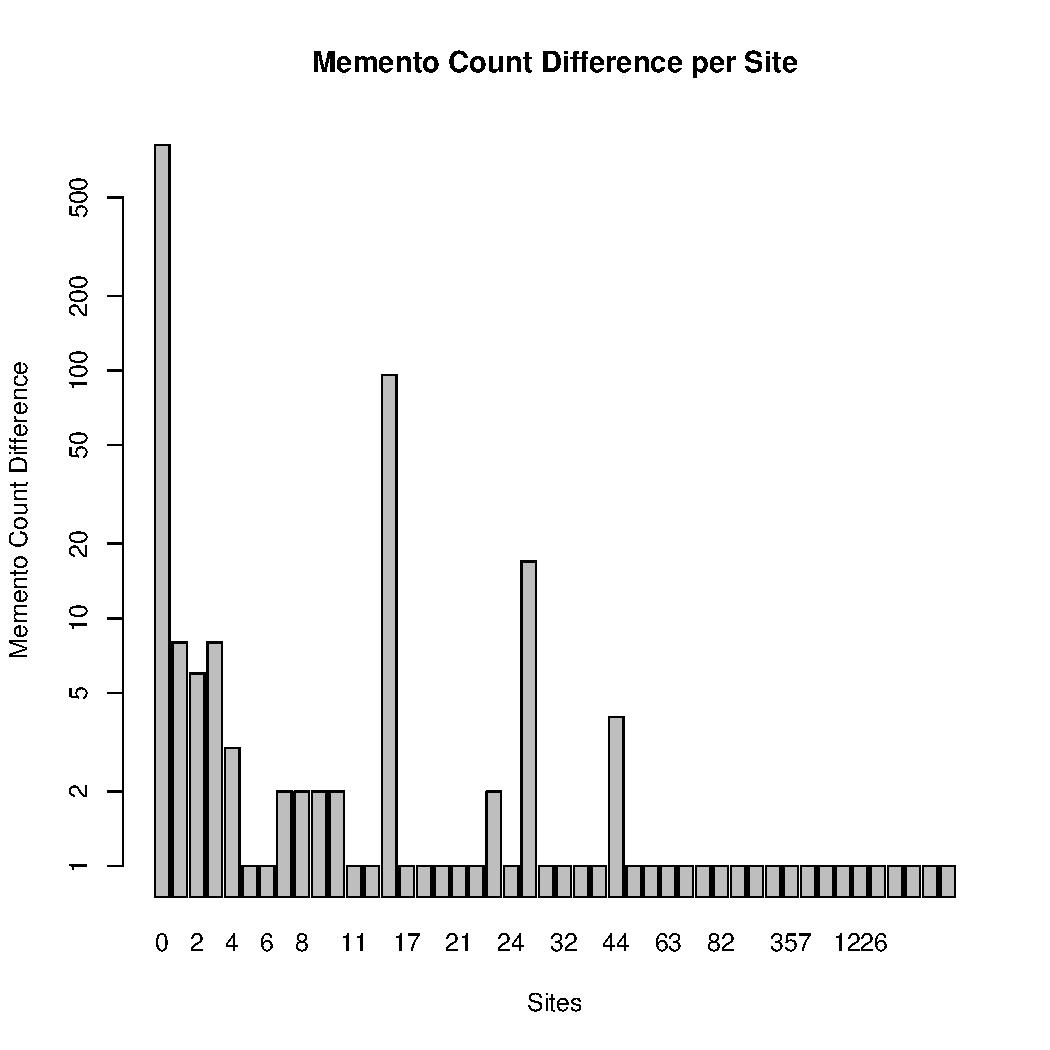
\includegraphics[scale=.85]{q3/histogram.pdf}}
\caption{Histogram of Mementos Count Difference}
\label{fig:hist_ss}
\end{figure}
